Originally posted at
\url{http://vinipsmaker.wordpress.com/2013/07/22/splines-extraction-on-kopf-lischinski-algorithm-part-0/}
on \formatdate{22}{7}{2013}.

\subsection{Generalized Voronoi diagram generation}

Well, a Voronoi diagram is a black box where you put some points (the seeds) and
you get some polygons (the cells). Each polygon contains all points that are
closer to its seed than any other seed. There is a
\href{http://en.wikipedia.org/wiki/Voronoi_diagram}{good article on Wikipedia}
and I won't explain any further.

Kopf-Lischinski algorithm executes a bunch of operations on a graph and it uses
a Voronoi diagram to extract a visual representation from this graph. The
simplest form of a Voronoi diagram works with 2D points-seeds, but we have
higher-dimentional Voronoi diagrams, Voronoi diagrams using different distance
functions and even Voronoi diagrams using complex non-points seeds. We are
interested in these Voronoi diagrams using complex non-points seeds.

The below image has a representation of the output graph of the Kopf-Lischinski
algorithm and its Voronoi diagram representation. The graph nodes are
represented by circles, where nodes with the same color are similar and usually
are connected. The connections of the nodes are represented by green lines.

\begin{figure}[H]
  \centering
  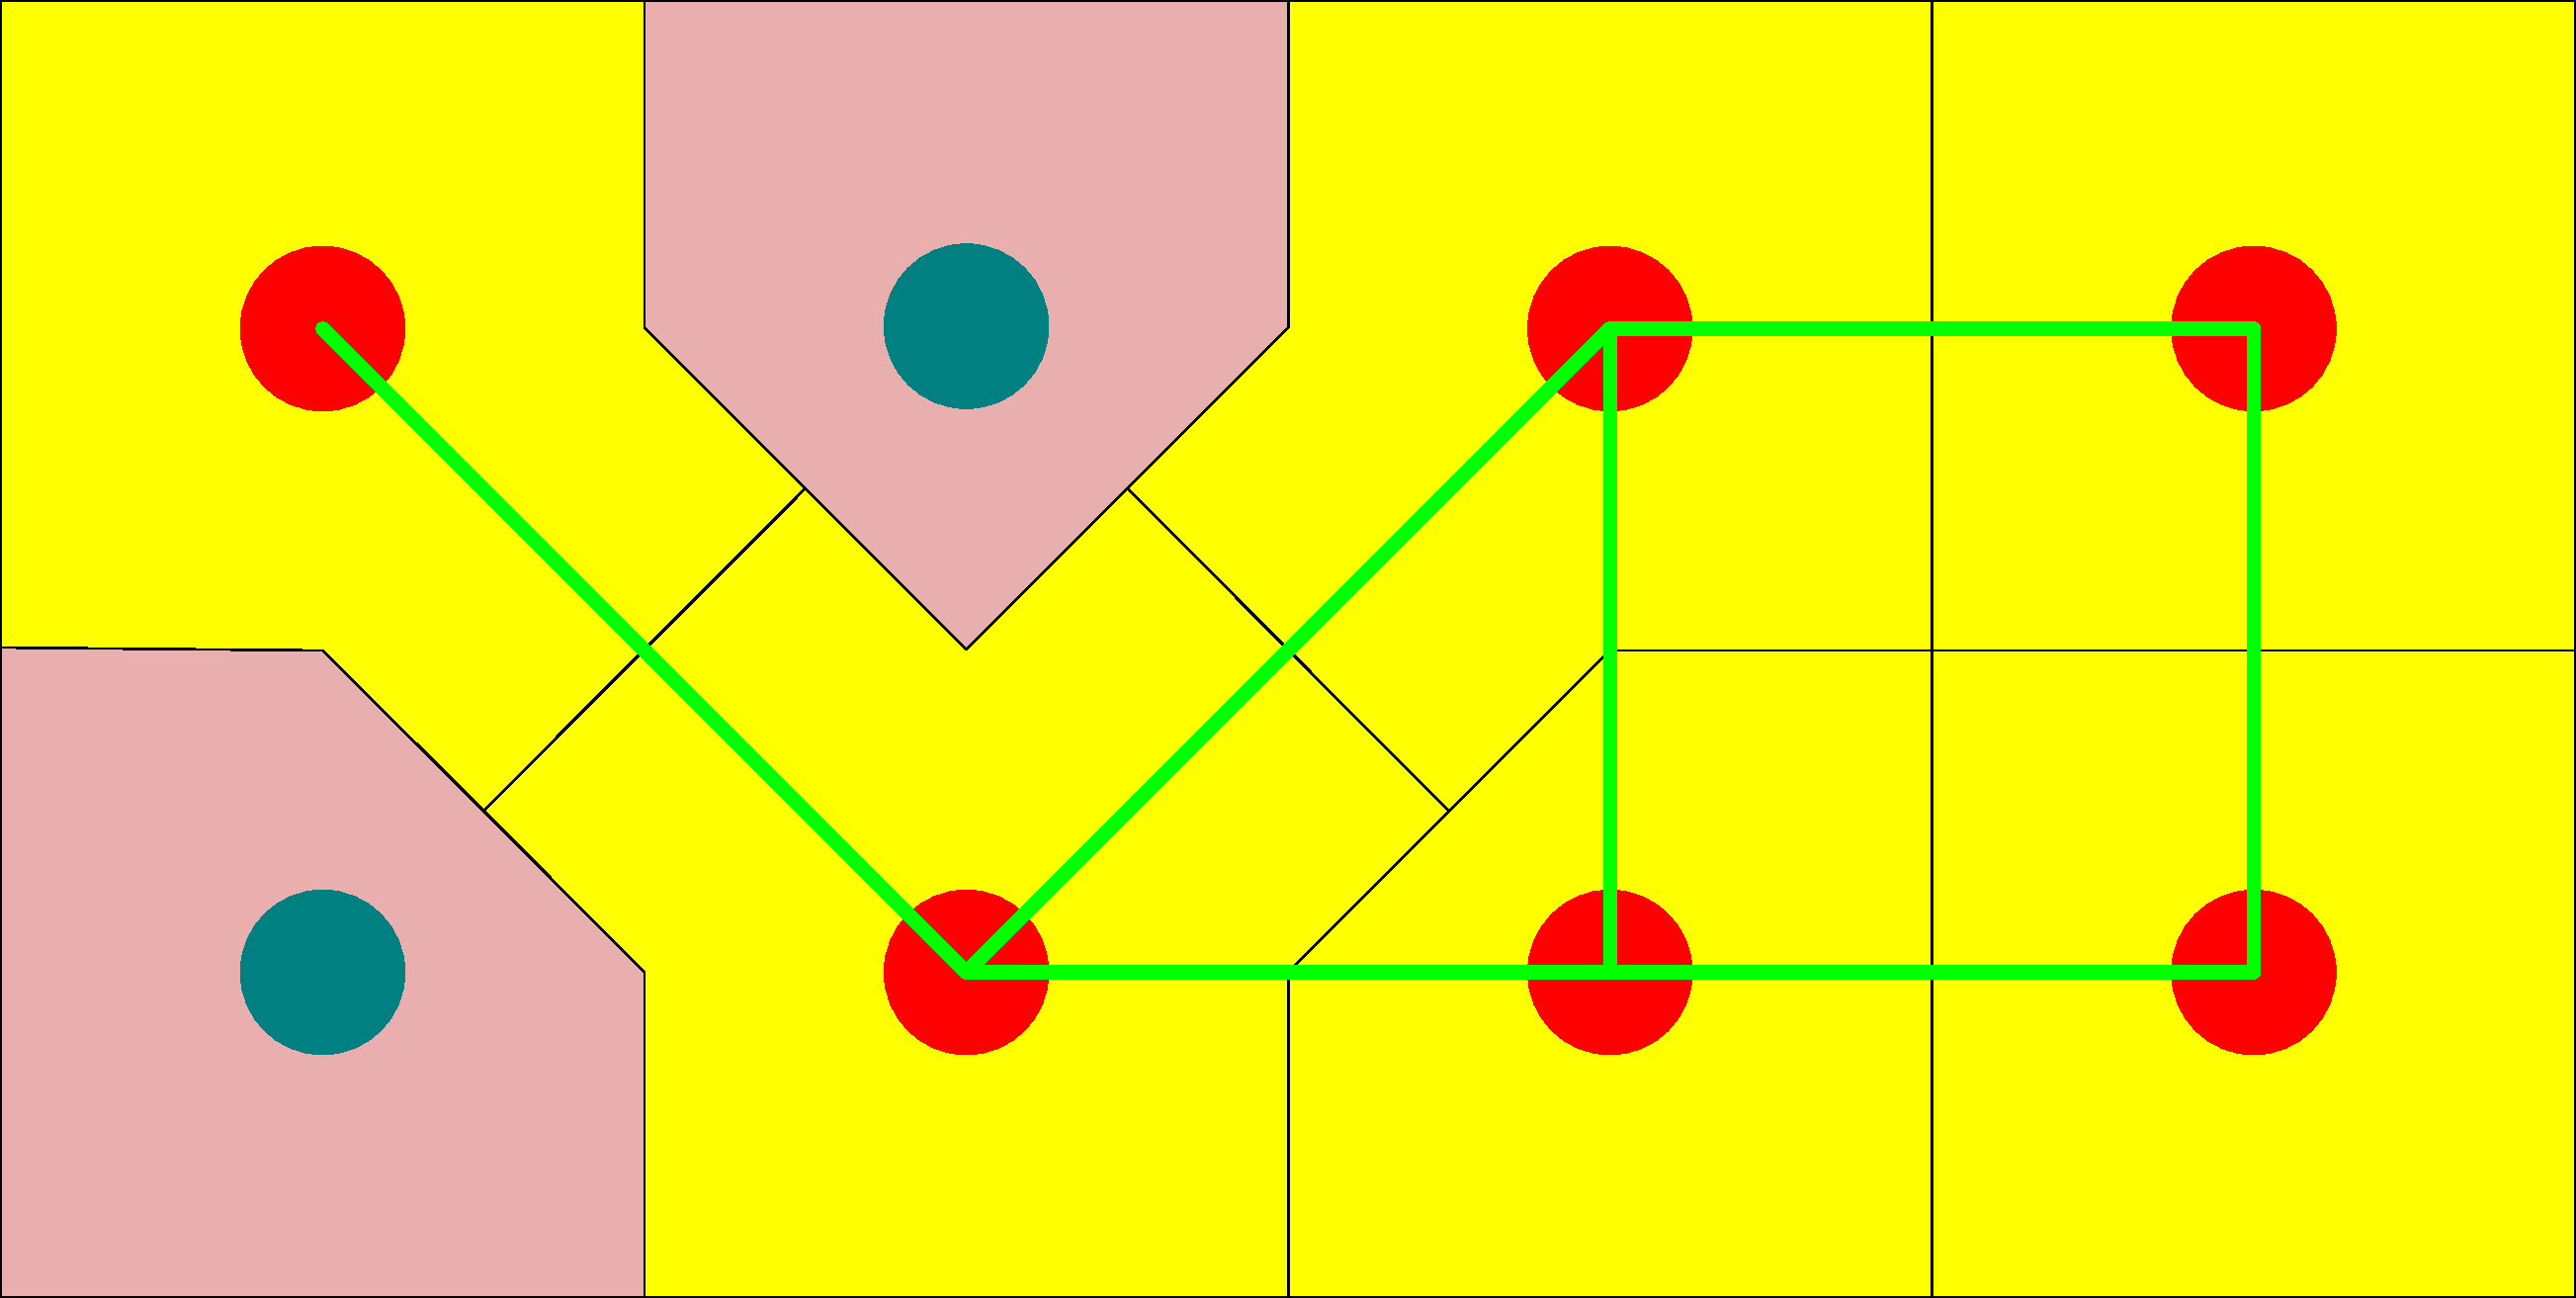
\includegraphics[width=0.8\textwidth]{assets/accurate_voronoi.pdf}
  \caption{An accurate generalized Voronoi diagram}
\end{figure}

The generalized Voronoi diagram is visual --- there is no special meaning to
explain it in the previous image. The seeds of this diagram aren't points, they
are line segments. You just need to break a green line in two and add each half
to its containing cell. You can note that some polygons aren't
\href{http://en.wikipedia.org/wiki/Convex_polygon}{convex}.

The graph used as input has certain constraints that enable us to use some
simple and fast operations instead of a
\href{http://en.wikipedia.org/wiki/Fortune\%27s_algorithm}{full-featured and
complex algorithm}.

If a Voronoi cell is a polygon containing all points that are closer to its seed
than any other seed, we can determine the edge of a Voronoi cell by the midpoint
of two adjacent seeds. If we generate a vertex for each of its 8 directions, we
will get an accurate Voronoi diagram.

\begin{figure}[H]
  \centering
  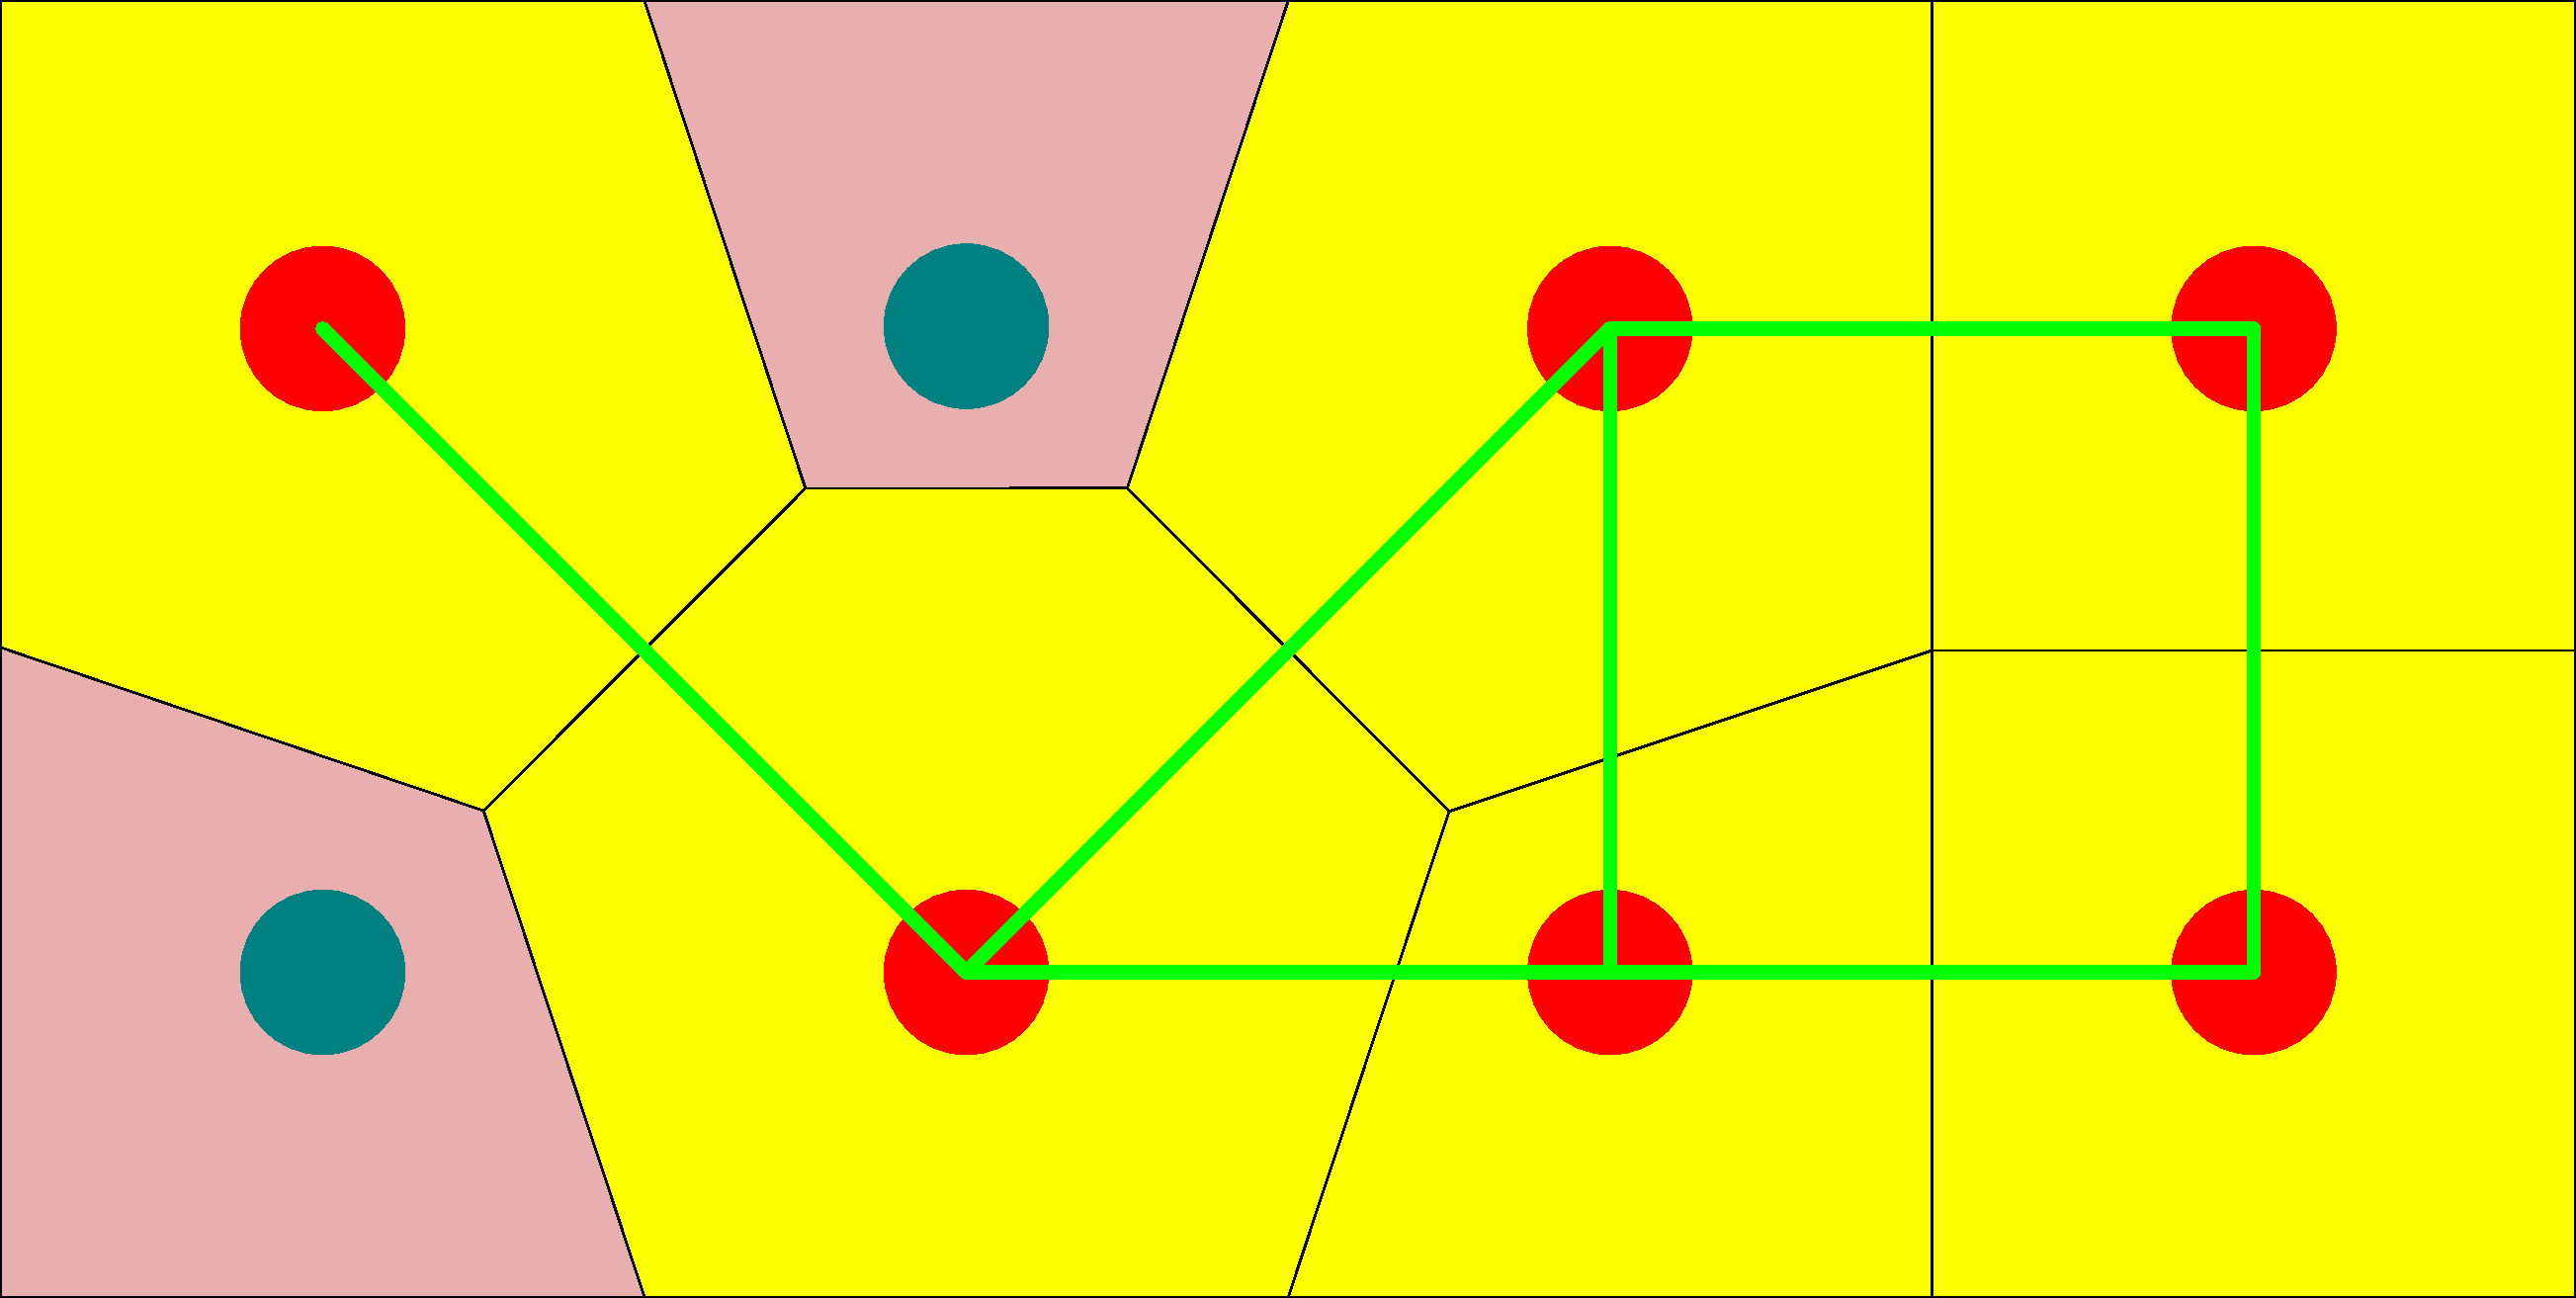
\includegraphics[width=0.8\textwidth]{assets/voronoi.pdf}
  \caption{A simplified generalized Voronoi diagram}
\end{figure}

We can get a simplified Voronoi diagram by forgetting about the top, bottom,
left and right vertices (if we just generate the diagonal vertices). The
simplified version doesn't contain
\href{http://en.wikipedia.org/wiki/Concave_polygon}{concave polygons}.

The act of generating diagonal vertices is more complex than the act of
generating the other vertices. We need to check if there is a connection with
the other cell and, if this connection exists, generate two vertices. If the
connection doesn't exist, we generate a single vertex, but its position depends
on the existence of a connection between its neighbors. Look the following
figure.

\begin{figure}[H]
  \centering
  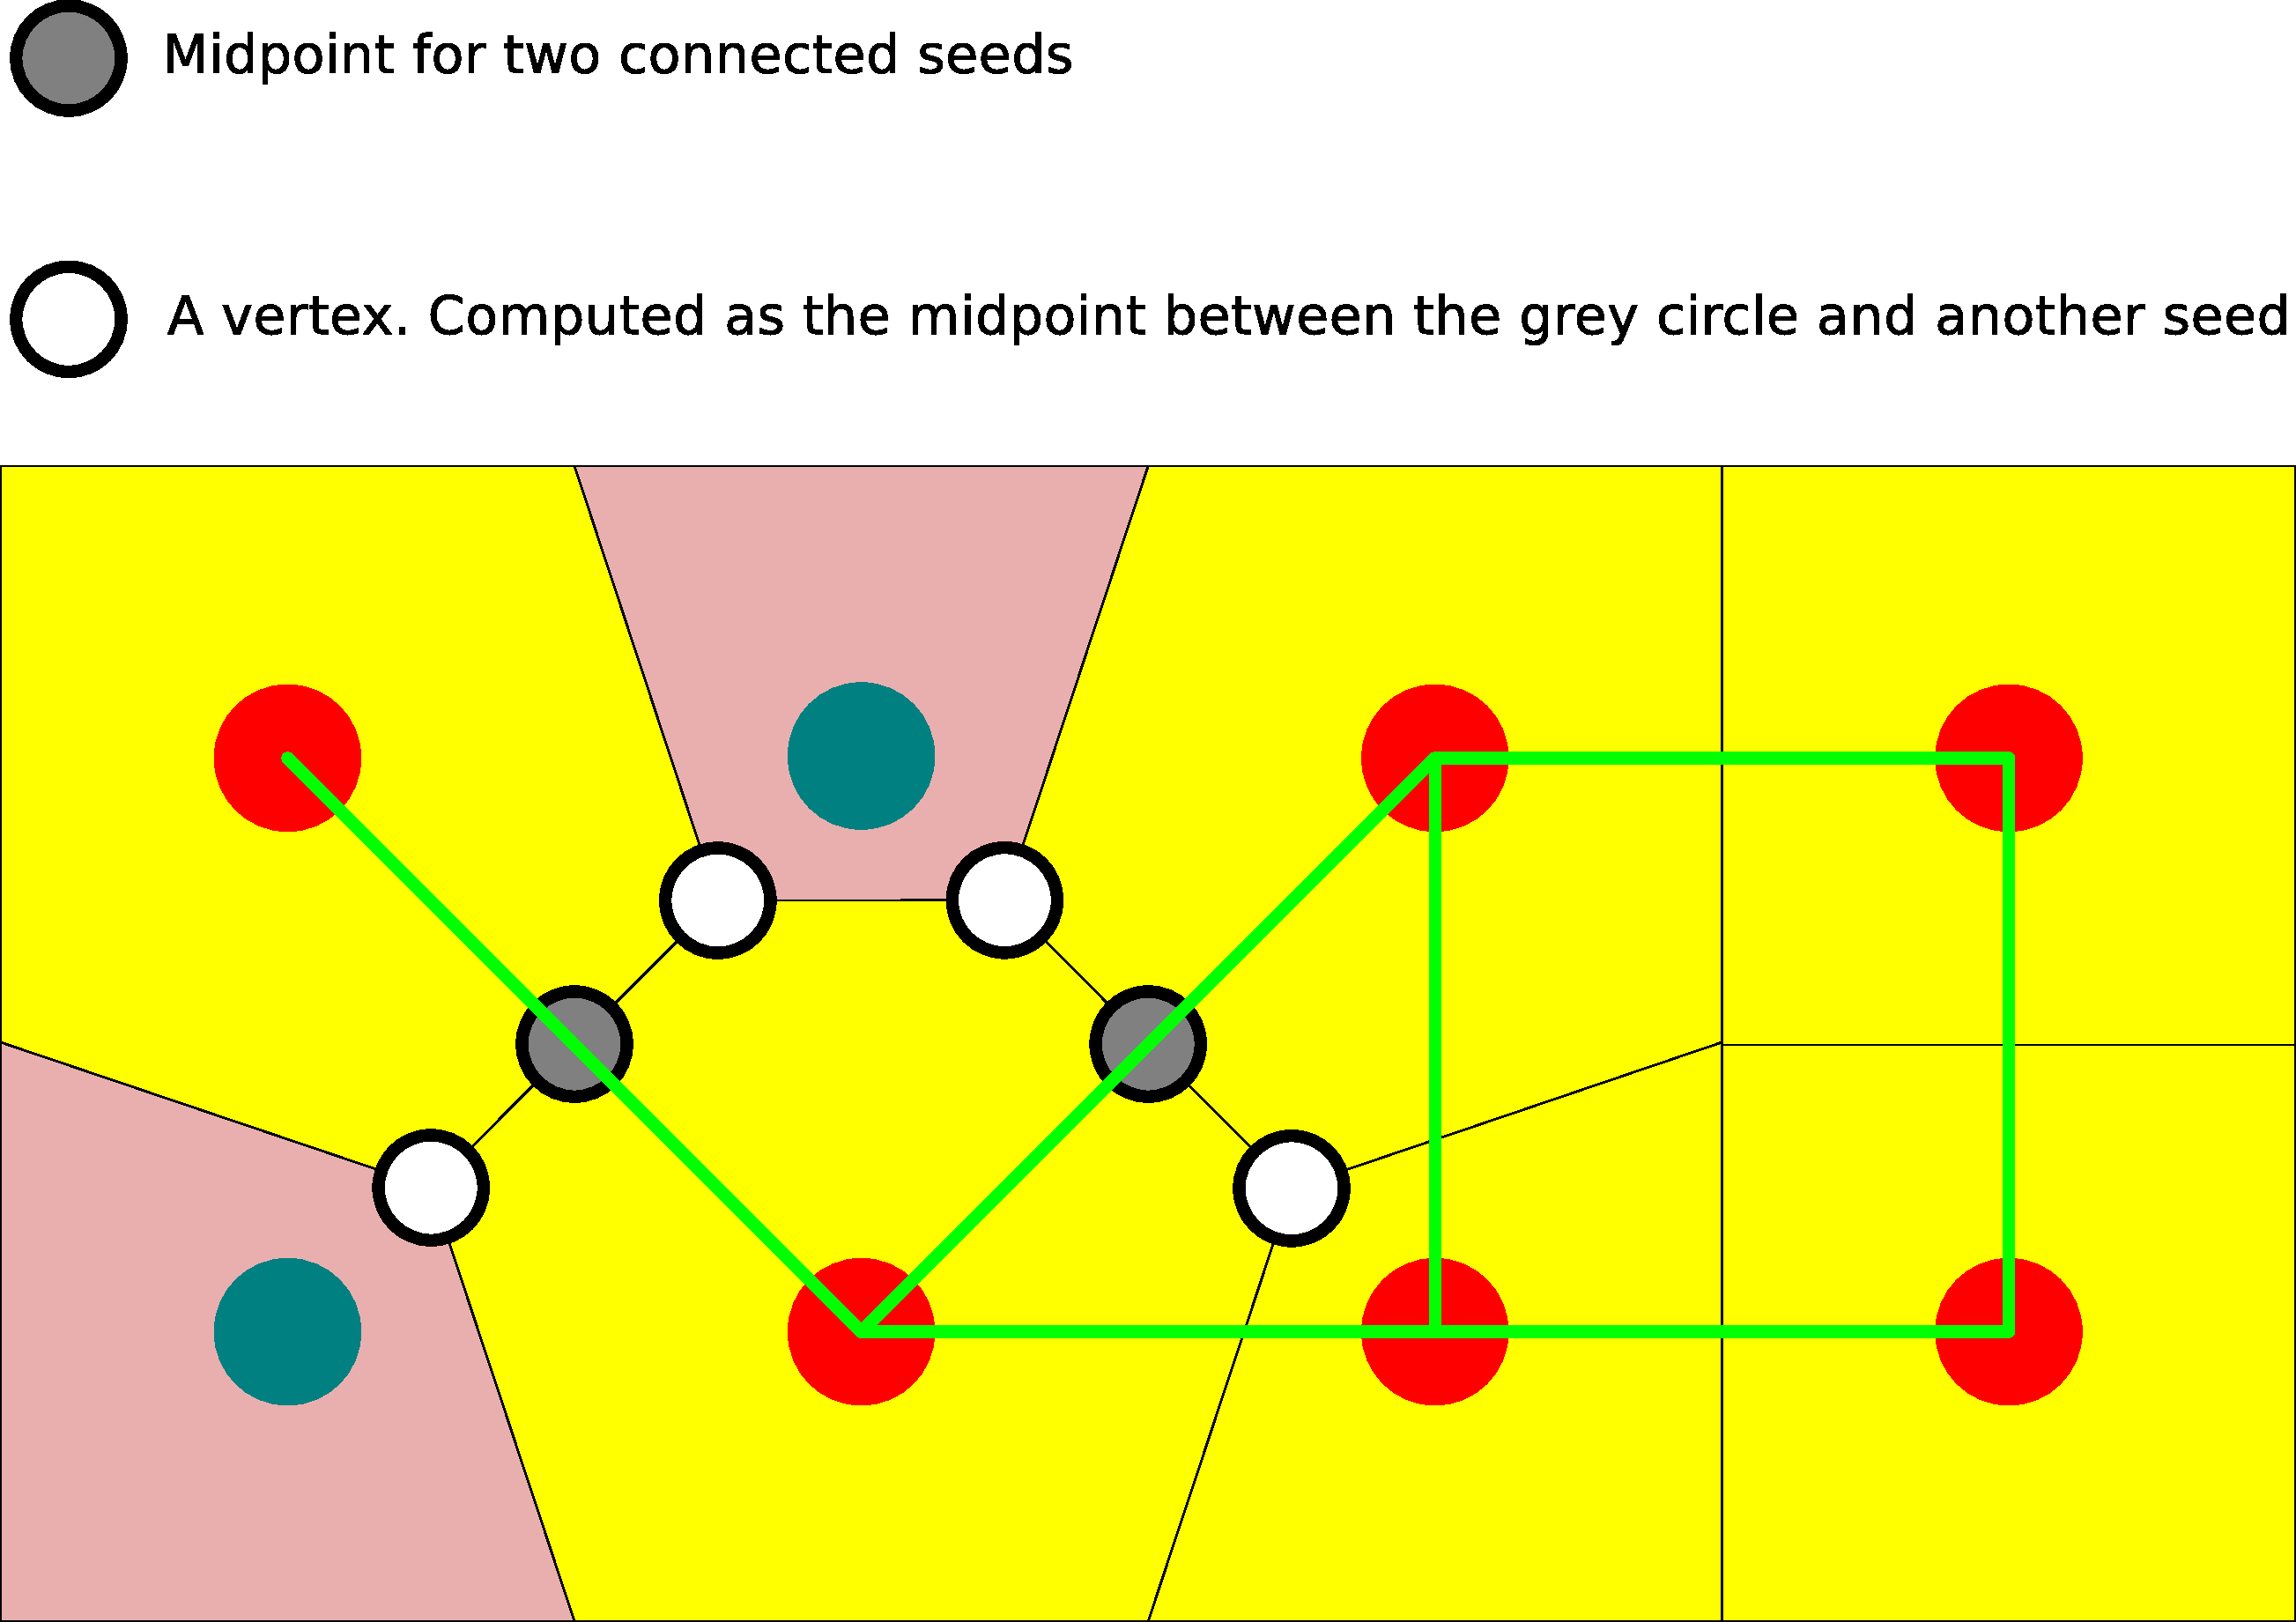
\includegraphics[width=0.8\textwidth]{assets/voronoi2.pdf}
  \caption{A simplified generalized Voronoi diagram (detailed)}
\end{figure}

All information we need to generate the Voronoi diagram is located within its
neighbors and the only extra tool we need to generate the points is the midpoint
procedure.

\subsection{Metadata extraction}

When we generate B-Splines using Kopf-Lischinski algorithm we need a way to
separate points that create sharp corners and smooth points. The Kopf-Lischinski
algorithm has techniques just to handle this issue. In libdepixelize, the point
smoothness computation and Voronoi generation are merged in one single phase.
This is the phase where we can gather lot of info about the graph and we can
propagate the smoothness data to later phases.

One note about the algorithm of this ``metadata extraction'' section is that
some points will disappear during polygon union and we don't care if the
metadata about these points is accurate, then we can simplify the algorithm
exploring this property.

Unfortunately (for the implementer only), graph nodes of different colors can be
grouped and if we don't intend to discard this \emph{extra color information}
(an extension of Kopf-Lischinski on its own), a special care must be taken to
handle these nodes. libdepixelize has some extensions that are documented later
in this document. But for now, to ease explanation, we consider only cells of
equal colors can be connected.

The below image has some features that will be citated in this subsection to
explain how the algorithm works:

\begin{figure}[H]
  \centering
  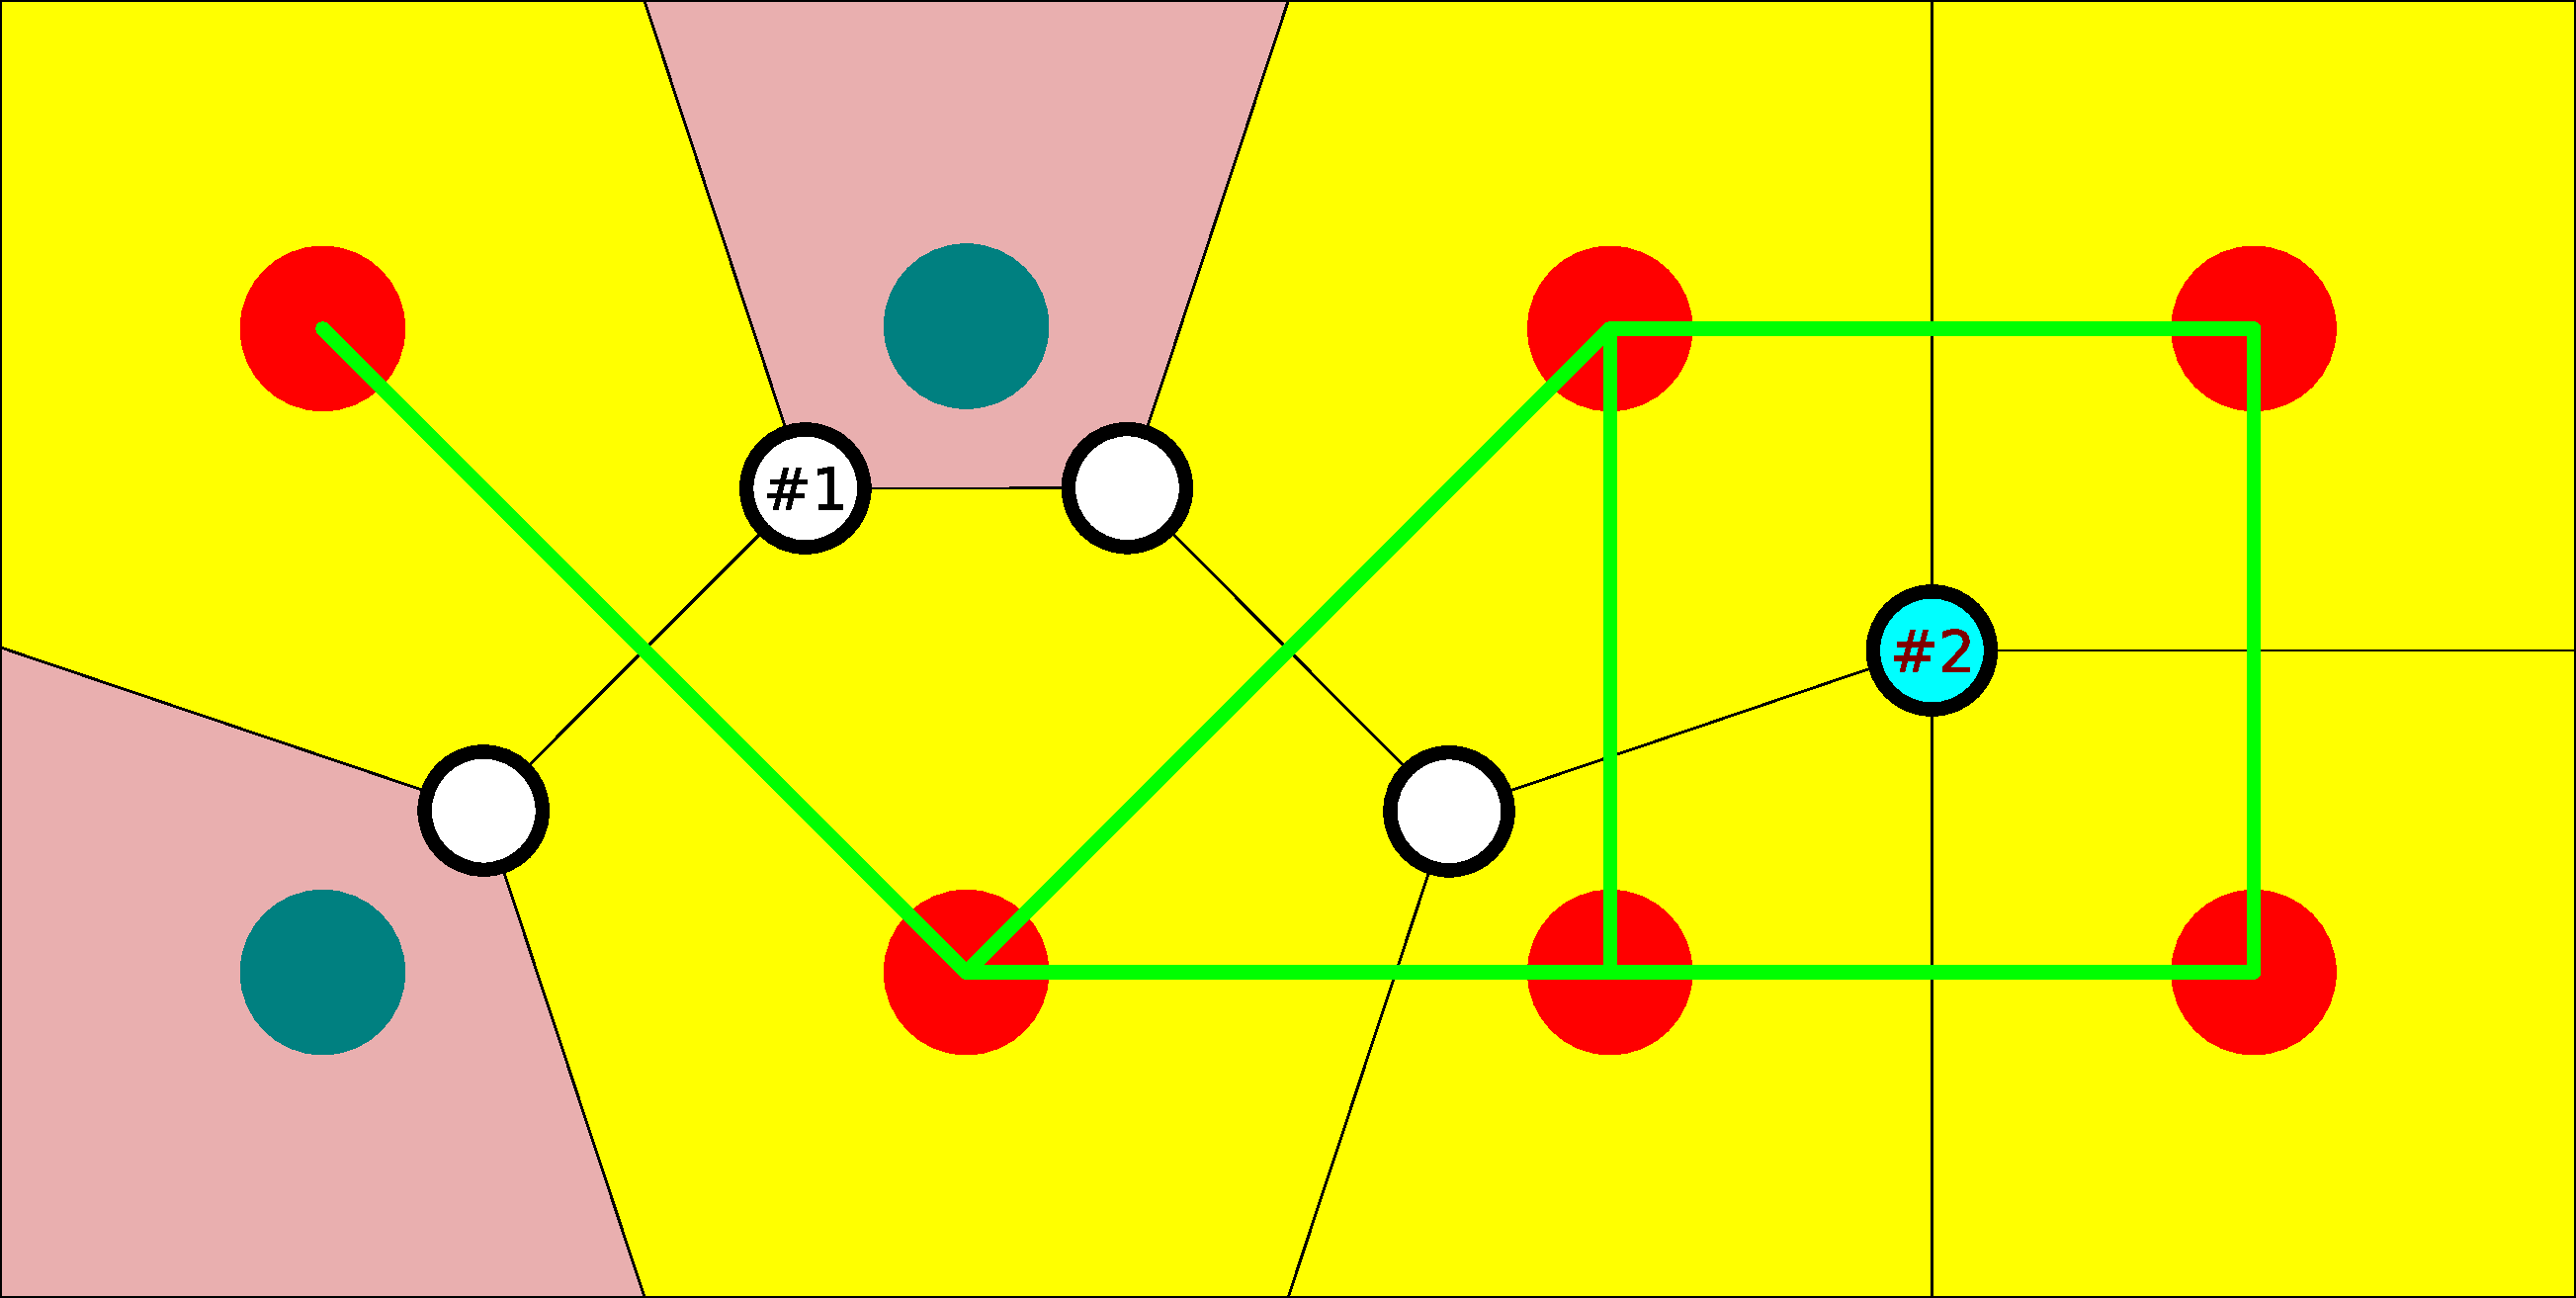
\includegraphics[width=0.8\textwidth]{assets/voronoi3.pdf}
  \caption{Vertex types}
\end{figure}

There are two types of vertices generated in this special Voronoi diagram:

\begin{itemize}
\item White type: The type of the one labelled with ``\#1''. Node ``\#1'' is
  contained by three cells, one purple and two yellows. The two yellow cells
  will be merged during polygon-union. There are two possibilities for the
  remaining cell in this kind of node:
  \begin{itemize}
  \item When it has the same color. Then the node will disappear during
    polygon-union and we don't care about its \emph{smoothness} attribute.
  \item When it has a different color. Then we say it is a valence-2 node.
  \end{itemize}
\item Cyan type: The type of the one labelled with ``\#2''. This type of node can
  appear in the border of the image and isn't smooth or in the center of 4 cells
  and its smoothness isn't predictable in advance. If it appears in the center
  of four cells, then:
  \begin{itemize}
  \item It can be in the middle of 4-connected cells and we don't care about its
    \emph{smoothness} attribute, because this node will disappear.
  \item It can be in the middle of a valence-2 node and will be smooth.
  \item It can be a valence-3 node and things start to get complex. After the
    polygon union, this node will be part of three different polygon and only
    two of these three nodes will share the same value for the \emph{smoothness}
    attribute.
  \end{itemize}
\end{itemize}

With these problems explained, it's time for the algorithm! The algorithm is
kind of repetitive (if we iterate the bottom-right node, compare with bottom and
right cells, then do all it again, but use nodes of different
directions\ldots{}), but the principle is the same for all ``repetitive'' code,
then only the important parts are documented here. If you really want to see the
whole thing, see appendix \ref{smoothness_code_appendix}.

\begin{figure}[H]
  \centering
  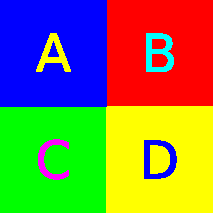
\includegraphics[width=0.8\textwidth]{assets/layout.pdf}
\end{figure}

The above image represents the analysed data in the following code example,
except for the fact that we don't know what are the colors of the cells. We are
iterating on the middle point of the image and the current iterated cell is cell
A. The algorithm also uses the concept of \emph{shading edge} and \emph{contour
edge} described in Kopf-Lischinski paper.

\lstinputlisting[language=C++,frame=single]{assets/code/smoothness.cpp}
